%%% -*-LaTeX-*-

\chapter{The Multi-cluster Trading Mechanism}

As the adoption of multi-cluster environments accelerates and the
infrastructure continues to evolve to support more use cases, we are presented
with an opportunity to build tools on top of that and leverage the existing
networking innovations to optimize how clusters interact in a multi-cluster
environment. 

In this chapter we present the system design. We first discuss how we designed
the trader to be minimally intrusive to local cluster scheduling. Then we
discuss the layout of the trader itself and the use of user-defined policies. 

It is possible to increase cluster resource utilization, decrease average job
completion time, and/or reduce average cost by providing clusters with a
resource trading mechanism allowing the virtual sharing of resources across
clusters. 

\begin{figure}[H]
    \centerline{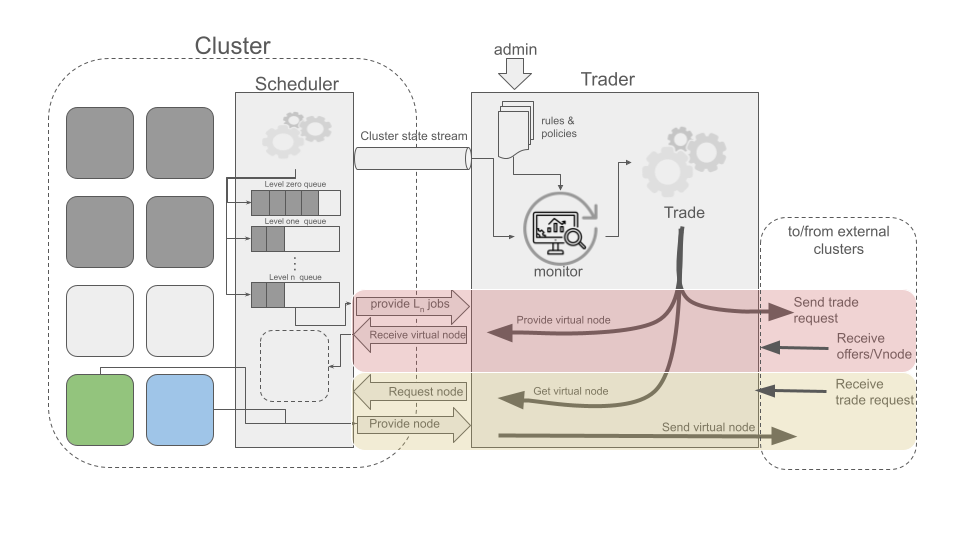
\includegraphics[scale=0.4]{figures/system-diagram}}
    \caption{System design showing the various compononents of the trader, and a snapshot of the cluster. }
    \figlabel{fig2}
\end{figure}

\section{Role of Scheduler in the mechanism}

Cluster scheduling have been widely studied, and continues to be a hot topic
with more innovations coming in. We don't aim to replace the well established
scheduling algorithms that clusters use. Our mechanism requests information
from the scheduler to operate on it's own. This information is limited and
depends on the policies the user is running. The overhead on the scheduler is
thus supplying the trader with the required cluster state data, which is
already being reported in current cluster schedulers. 

Cluster state encompasses all required metadata of the cluster for the trader
to make trading decisions. This includes but is not limited to average wait
time, average cost of compute/memory, average utilization. 

The other requirement for the scheduler is actually scheduling the jobs on the
foreign cluster. By the end of the trade, the scheduler will be presented with
a virtual node, with actual resources in the foreign cluster, to schedule. This
bolsters our design decision of keeping trading minimally intrusive to the
scheduling module. However, it would be advised to use this node as fast as
possible due to its limited time span. This would be further discussed in the
implementation section.  

% add figure of scheduler or algorithm 
[ADD FIGURE OF SCHEDULER DESIGN / ALGORITHM]

Although a specific scheduling algorithm is not required for our mechanism to
run, we noticed that delay scheduling would be a good fit for our mechanism due
to its focus on locality. With the highest level queue including the jobs that
are more likely going to be scheduled far from their data/resources, these jobs
would hypothetically incur the least reduction in performance when scheduled in
a foreign cluster. These jobs also have the highest wait times, keeping
fairness at check. 

Of course, more analysis could go in deciding what jobs would better fit being
exported to other clusters like jobs demanding less communiication with other
jobs in the cluster, jobs with less data dependency, ..., but this is out of
scope of this thesis.
% research idea: data locality-aware scheduling research is trying to get the
% jobs scheduled next to data, no study i encountered actually socres the
% sensitivity of the jobs in relation to other jobs in the cluster. (probably
% for fairness concerns) but might be an interesting project to work on. 

%This presents us with a clean heuristic when calculalting resources needed for
%trading. As the level of the of what to include in our 

\section{Policies}

% Policy intro
Policies are created to optimize a specific performance metric, acting as knobs
to tune the mechanism and update it as cluster requirements change. They are a
set of rules that dictate how each cluster handles trading. Policies are
pluggable and mutable, meaning each cluster can implement its own request and
receive policy, and dynamically update it as requirements or conditions change.
Policies are two types, incoming and outgoing. 

\subsection{Incoming} 

Incoming policies set the rules for accepting resource requests from foreign
clusters. The mechanism consults the policy, comparing the current cluster
state with the requested resources and concludes its decision.

% add figure for policy? or give an example??
[ADD FIGURE]

\subsection{Outgoing}

As the system continously monitors the cluster state, it makes sure the state
does not break any of the outgoing policies' requirements. Once that happens
the mechanism initiates the trading procedure. 

[ADD FIGURE]

\section{Trader}

The trader is the main component of the mechanism. As an orchestrator, K8s role
is to sync the actual cluster state with the declared desired state. This
involves spawning a new container if an old one died or scaling a service if it
gets more traffic. The trader plays a similar role, it is responsible for
keeping the cluster's state in sync with the declared desired state. The
desired state is declared through the user defined outgoing policies. Once the
current state of the cluster breaks an outgoing policy, it initiates the
trading request algorithm. 
% add trading request algorithm
% Example Algorithm
\begin{algorithm}[H]
\caption{Trading Scheduling Algorithm - Requester}
\begin{algorithmic}
    \For{job in WaitQueue}
        \State $scheduled \gets ScheduleJob(job)$
        \If{$scheduled \neq True$ \&\& Policy(job) $==$ True} 
        \State $requestResources(job)$
        \EndIf
    \EndFor

    \For{job in ReadyQueue}
        \State $scheduled \gets ScheduleJob(job)$
        \If{$scheduled \neq True$}
        \State $WaitQueue \gets WaitQueue + job$
        \EndIf
    \EndFor
\end{algorithmic}
\end{algorithm}

The first step in the trading algorithm is determining the amount of resources
needed. First, the trader requests more information from the scheduler. The
scheduler is required to share a job's list with the trader. The trader in turn
uses the information provided to calculate the requested node size. The user
defined outgoing policy also dictates any additional constraints the trader is
required to adhere to. If the notion of a currency is established in the
multi-cluster environmnet, constraints would include a budget, as well as a
maximum price to pay for resources, which can be the price of renting out the
resources from the vendor, or a cost estimate anaylsis algorithm. 

After calculating the needed resources, the trader then broadcasts a contract
to all participating clusters, and waits for replies. After receiving approved
contracts, the trader approves the best contract, and receives the virtual node
information from the foreign trader. It then sends the virtual node for the
scheduler to start scheduling jobs on it.

\begin{algorithm}[H]
    \caption{Trading Scheduling Algorithm - Receiver}
    \begin{algorithmic}
            \State $ resources \gets BorrowRequest $ \Comment{Incoming from another cluster} 
            \If{$Policy(resources) = True$} 
            \State $sendAcceptRequest(job, cluster)$
            \State $prepareResources(resources)$
            \State $allowAccess$
            \EndIf
    \end{algorithmic}
\end{algorithm} 

The trader is also responsible for accepting/rejecting incoming requests. After
receiving a contract request, the trader consults the incoming policy and the
current cluster state, and decides whether to approve the contract. If the
trader gets picked by the foreign cluster, the trader then requests the needed
resources from the scheduler and sends the node information back to the foreign
trader.
\newpage


%Our mechanism offers bidirectional trading, allowing clusters to trade
%resources with one another. It also enables trading with multiple clusters, so
%clusters can trade resources with more than one cluster at a time.
%\label{sched-overhead} The following algorithms show a simple representation
%of the system, with resource utilization as the optimized-for metric:
%\label{example}
